% Updated from completed, frozen experiments on 2026-11-03.
% Historical evaluation text is preserved as comments below the active section.
\section{Experimental Protocol and Supplementary Evidence}
\label{app:evaluation}
\noindent\textbf{Correspondence: Section~\ref{sec:evaluation}.} This appendix preserves the extended model, intermediate steps and supporting interpretation behind the corresponding main-text section.


\label{detail:sec:evaluation}

The evaluation connects the controller analysis to three distinct questions:
whether the continuous-clock implementation respects the PI calibration;
whether the nonlinear reference trajectories agree with the mathematical
analysis; and whether the proposed controller offers a measurable benefit
against independently tuned PI under shared delivery disturbances. We
separate matched-gain mechanism checks from equal-budget controller
selection, and reference-model certificates from actual Callisto measurements.

\subsection{Experimental design and continuous-clock execution}
\label{detail:subsec:eval_design}

All actual experiments use the continuous-phase Callisto realization of
Section~\ref{detail:sec:fpi_controller}. Oscillator phases evolve continuously,
integer frame crossings determine buffer events, and measurements and
correction applications are scheduled by each node's local phase. There
is no common physical polling grid. Table~\ref{detail:tab:eval_setup} gives the
nominal plant; the startup stress study changes the intrinsic frequencies
and reconstructs the associated negative-time histories explicitly.

\begin{table*}[t]
\caption{Nominal actual-Callisto configuration. Time is in physical reference
ticks except where local ticks are explicitly stated. Controller parameters
selected for independent tests are listed separately in
Table~\ref{detail:tab:eval_selected_gains}.}
\label{detail:tab:eval_setup}
\centering
\begin{tabular}{@{}ll@{}}\toprule
Parameter & Value\\\midrule
Topology & Three-node bidirectional triangle; six receiving buffers\\
Intrinsic frequencies $\omega^u$ & $(1.0002,0.9998,0.9999)^\top$; initial spread 400 ppm\\
Initial phase; base frequency & $0.1$ at every node; $\omega_{\rm base}=29999/30000$\\
Capacity; initial occupancy; target & $C=2048$; $\beta_e(0)=\beta_e^*=1024$ frames\\
Initial in-flight frames; marking & 20 per channel; 1044 in the recorded convention\\
Nominal path delay & 20\\
Polling; control-execution delay & $p=1000$; $d_{\rm ctrl}=10$ local ticks\\
Execution constraints & $|u_i|\le0.01$; guards enabled; reserve zero; no anti-windup\\
Control law & Native integrate-first PI or the complete incremental 25-rule Fuzzy law\\
Other mechanisms & Observer and supervisory mode switching disabled\\
Disturbance onset & $t_{\rm on}=2\times10^6$\\\bottomrule
\end{tabular}
\end{table*}

\paragraph{Evidence groups and data separation.}
The implementation check, M0, contains six matched pairs, or 12 actual
runs. An earlier fixed-preset burst campaign, M2, supplies a separate
mechanism diagnostic. The earlier fixed-preset random campaign, M3, is
development evidence and supplies no seeds to the new independent tests.
Its fixed-preset comparison did not support lower Fuzzy RMS against
moderate PI; the new study asks the different question of independently
selected controllers under an equal evaluation budget.
The new training study charges 192 slots, including four verified cached
M2 evaluations and 188 new actual runs. Selection is frozen before 186
new held-out runs. A separately registered slower-disturbance study adds
107 actual runs, including its engineering pilots, and the startup
study adds six. Its 32 synchronous fluid-reference trajectories are
reference calculations, not additional actual runs. Old data, infeasible
candidates and repair records are retained in the evidence archive.

\paragraph{Shared delivery inputs.}
All controllers receive identical externally generated desired-latency
profiles within each comparison, verified by content hashes. Delay is
20 before onset, including the negative-time prehistory. Ordered arrivals
use the causal running-maximum envelope of
Section~\ref{detail:sec:fpi_controller}; a delay decrease may release an ordered
batch. The model does not impose a finite serialization rate.
For bounded random latency, the desired delay is $20+z_m$, where
\begin{align}
 z_0&=5\varepsilon_0,\nonumber\\
 z_m&=r_z z_{m-1}+(1-r_z)5\varepsilon_m,
 \quad r_z=e^{-1},\quad\varepsilon_m\sim\mathcal U[-1,1].
 \label{detail:eq:eval_random_profile}
\end{align}
Thus desired delay remains in $[15,25]$. The index $m$ counts physical
profile updates on a grid of spacing $T_c$, independently of controller
polling. Here $T_c$ denotes a profile-update interval, not an exactly
measured correlation time. The original two regimes use $T_c=1000$
and $10000$; the later confirmation study uses $100000$.

\subsection{Metrics, admissibility and comparison windows}
\label{detail:subsec:eval_metrics}

For $n$ nodes, let $\bar\omega(t)=n^{-1}\sum_i\omega_i(t)$ and define
the instantaneous across-node root-mean-square (RMS) disagreement as
\begin{align}
 \sigma_\omega(t)&=\sqrt{n^{-1}\sum_i[\omega_i(t)-\bar\omega(t)]^2},\nonumber\\
 \sigma_{\rm ppm}(t)&=10^6\sigma_\omega(t)/\omega_{\rm unit},
 \qquad\omega_{\rm unit}=1.
 \label{detail:eq:eval_disagreement_amplitude}
\end{align}
Parts per million (ppm) use the fixed normalized frequency unit, not
$\omega_{\rm base}$. For a physical-time window $W=[a,b)$ of duration
$T_W=b-a$, report
\begin{align}
 R_W&=\sqrt{T_W^{-1}\int_W\sigma_{\rm ppm}(t)^2\,dt},\nonumber\\
 I_W&=\int_W\sigma_{\rm ppm}(t)\,dt,
 \qquad P_W=\sup_{t\in W}\sigma_{\rm ppm}(t).
 \label{detail:eq:eval_frequency_metrics}
\end{align}
The integral absolute error (IAE) $I_W$ integrates RMS amplitude, rather
than the mean absolute node deviation. Frequency moments use complete
held-frequency intervals weighted by their physical durations.
The actual pairwise spread $\Delta_\omega=\max_i\omega_i-\min_i\omega_i$
is recorded separately. Although
$\Delta_\omega\le\sqrt{2n}\,\sigma_\omega$ pointwise, window RMS alone
does not establish a maximum transient-spread bound.

Buffer excursion, minimum two-sided headroom and mean command total
variation (TV) are
\begin{align}
 B_W^{\rm obs}&=\max_e\sup_{t\in[a,b]}|\beta_e(t)-\beta_e^*|,\nonumber\\
 H_W^{\rm obs}&=\min_e\inf_{t\in[a,b]}
                         \min\{\beta_e(t),C-\beta_e(t)\},
 \label{detail:eq:eval_buffer_metrics}\\
 \mathrm{TV}_W&=n^{-1}\sum_i
       \sum_{k:\,a\le t^a_{i,k}\le b}|u_{i,k}-u_{i,k-1}|.
 \label{detail:eq:eval_tv}
\end{align}
Buffer statistics reconstruct all integer crossings and ordered arrivals,
grouping simultaneous events and including the endpoint state. Sparse
plot samples do not determine extrema. TV includes both endpoints under
the frozen convention, so adjacent-window activities cannot be added
without treating the shared endpoint. TV measures command activity,
not hardware energy. Requested and applied corrections, saturation,
gate events, positive frequency and data-phase progress are checked
separately.

Before each post-centering disturbance, three consecutive $10^5$-tick
windows ending at onset must satisfy disagreement RMS at most 2 ppm,
each buffer's absolute mean bias at most two frames and standard
deviation at most one frame, common-frequency temporal standard
deviation at most 1 ppm and three-window mean range at most 1 ppm,
with positive progress and no intervention. These are finite
engineering centering criteria, not exact equilibrium. A training
candidate failing the same criteria in any required case remains
infeasible and consumes its assigned budget.

The original-regime tests use $W=[2\times10^6,4\times10^6)$ and tail
$[3.6\times10^6,4\times10^6)$. Each controller's own clean trajectory
is its same-parameter, nominal-delay counterfactual over the same
physical times. Common-frequency shift is reported relative to this
counterfactual, separately from relative synchronization. Strict
recovery requires the centering criteria for three consecutive windows
and a window-mean common frequency within 2 ppm of own clean. A return
not observed by the specified endpoint is right-censored, not assigned
a recovery time of zero or interpreted as permanent nonrecovery.

\subsection{Implementation and nonlinear-reference validation}
\label{detail:subsec:eval_implementation_reference}

M0 checks Proposition~\ref{detail:prop:fpi_equivalence} by replacing the Fuzzy
surface with its calibrated linear counterpart $F_0$, without changing
the continuous plant. Six pairs cover polling periods 100 and 1000,
initial frequency spreads 35 and 400 ppm, and capacity/target settings
$(2048,1024)$, $(512,128)$ and $(512,384)$ over $2\times10^5$ ticks.
Across 19,800 paired updates, the maximum correction difference is
$5.29\times10^{-18}$; physical/data phases, measurement vectors and
saved buffer counts agree, without saturation or guard intervention.
This checks initialization, integration order and gain mapping. It does
not replace the complete nonlinear law in the performance experiments.

The original 25-rule law is also evaluated directly on the synchronous,
zero-delay reference of Section~\ref{detail:sec:btd_reference}, with 2000
post-bootstrap updates. At the prescribed moderate-gain initialization,
the fluid buffer peak is approximately 17.314056818 frames, maximum
$|X|+|Y|$ is 0.090130790, maximum absolute correction is
$3.21398377\times10^{-4}$, and no contraction-envelope violation is
observed. Physical frequencies stay in $[0.9998,1.0002]$ including
startup. These finite numerical checks agree with the analysis; the
all-time comparison, Fuzzy below 17.315 versus PI approximately
23.403701 frames, follows from the interval-prefix and contracting-tail
proof in Theorem~\ref{detail:thm:btd_headroom}.

\paragraph{Rule verification.}
We reconstruct requested corrections from the saved inputs in all 299
new validation, slow-delivery and actual startup records. The maximum
residual is approximately $5.42\times10^{-20}$. This uses the complete
rule map and stored accumulator, not a sector surrogate. The earlier
M2 diagnostic additionally stays within $\Omega_5$, with observed
$\max(|X|+|Y|)=2.001888$, supporting application of
Proposition~\ref{detail:prop:fpi_central} to those measured inputs. This
diagnostic is retained separately from the independently selected
controllers: Fuzzy$_B$ reaches approximately 39.159 in the large
held-out burst. The full 25-rule law remains defined there, whereas
the central-region identity and the $\Omega_1$ reference witness do
not cover that whole trace. Same-input memory accounting is an
algebraic diagnostic, not an additional closed-loop $F_0$ experiment.

\subsection{Reference safety strata and actual startup transients}
\label{detail:subsec:eval_safety}

To vary initial mismatch without changing occupancy normalization,
capacity and targets remain fixed while
\begin{equation}
 \omega^u(s)=\frac{29999}{30000}\mathbf1
                 +s\frac{(7,-5,-2)^\top}{30000},
 \quad s\in\{0.5,1,2,4,8,16,32,64\}.
 \label{detail:eq:eval_stress_direction}
\end{equation}
Here $s$ is an initial-mismatch scale, with intrinsic spread $400s$ ppm.
The reference uses the matched moderate coordinates
$(k_p,k_i)=(2\times10^{-6},5\times10^{-11})$, synchronous zero-delay
fluid execution and $H=h=30000000/29999$. Its 32 trajectories comprise
two controllers, eight scales and both unprotected virtual and
$0.01$-clipped variants. Each includes the bootstrap and 2000 subsequent
zero-order-hold intervals. The initial certificate energy scales as
$V_1(s)=s^2V_1(1)$; input-domain, buffer, positive-frequency and correction
conditions are checked jointly.

The largest grid point satisfying the common sufficient conditions is
$s=2$. At $s=4$, both reference trajectories remain normal over the
record although the certificate no longer guarantees them. At $s=32$,
unprotected reference requests first require actuator clipping; at
$s=64$, both virtual reference buffer trajectories violate capacity.
Figure~\ref{detail:fig:eval_reference_grid} distinguishes measured virtual
peaks from sufficient bounds. Failure of a sufficient condition is
inconclusive, rather than a prediction of instability.

\begin{figure*}[t]
\centering
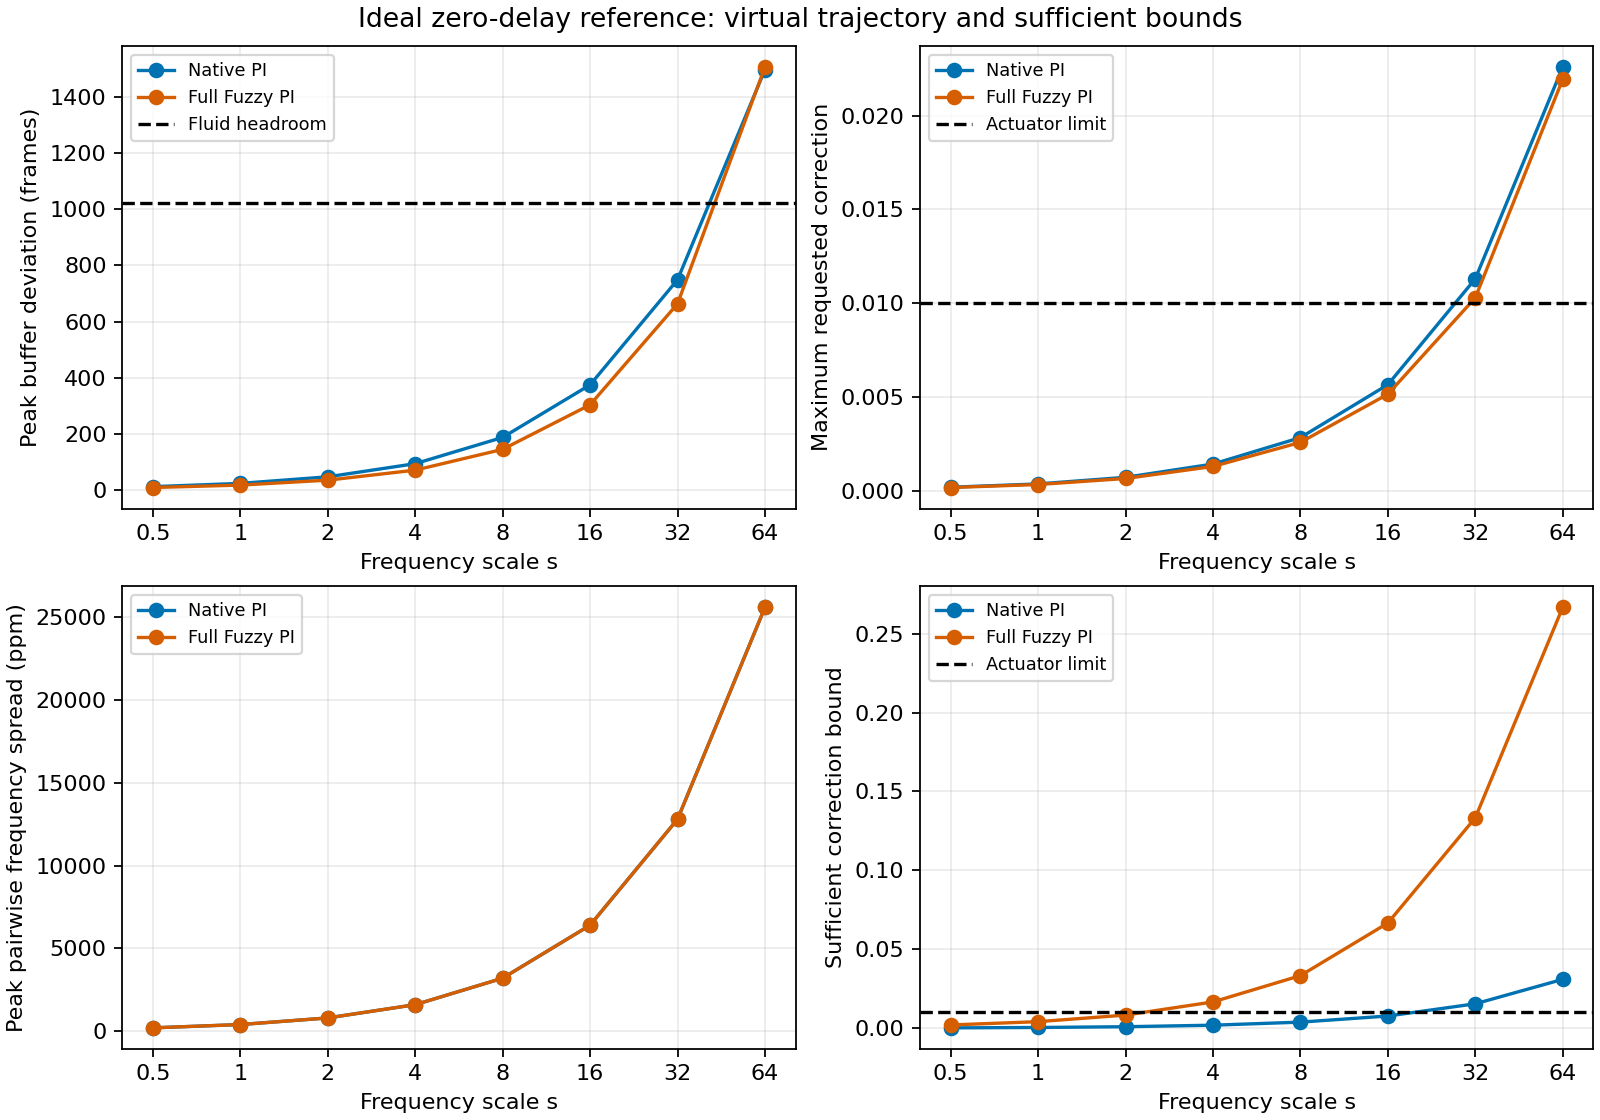
\includegraphics[width=0.97\textwidth]{images/evaluation_latest_20261103/reference_grid.png}
\caption{Synchronous zero-delay fluid-reference sweep at matched moderate
coordinates. Virtual trajectory peaks and analytical sufficient bounds
are distinct quantities. The dashed levels show fluid buffer headroom
and the correction limit; clipping and unprotected virtual trajectories
are archived separately. These are reference calculations, not actual
Callisto safety certificates.}
\Description{Four panels compare reference buffer peaks, requested corrections,
frequency spread and correction bounds over eight initial-mismatch scales.}
\label{detail:fig:eval_reference_grid}
\end{figure*}

Before running actual cases, the selection rule freezes three common
scales: 2, 4 and 32, representing certified, observed-safe uncertified,
and correction-constrained reference strata. Actual Callisto restores
path delay 20 and local polling/control delay 1000/10. Its locked
startup horizon is $2001H\simeq2.001067\times10^6$ physical ticks,
rather than the $4\times10^6$ used for the disturbance tests. This
shorter horizon is an execution-plan deviation from the earlier
completion instruction and limits the empirical safety observation
accordingly. The six cases are startup stress tests, not
post-centering disturbance tests.

\begin{table}[t]
\caption{Actual startup stress at matched moderate coordinates. Buffer
excursions include startup and all reconstructed events. Sat. counts
saturated control updates; every case has zero gate events and replay
mismatches.}
\label{detail:tab:eval_startup_safety}
\centering
\begin{tabular}{@{}rrrrr@{}}\toprule
 & & \multicolumn{2}{c}{Buffer excursion / frames} & Sat.\\
$s$ & Spread / ppm & PI & Fuzzy & PI / Fuzzy\\\midrule
2 & 800 & 47 & 37 & 0 / 0\\
4 & 1600 & 94 & 72 & 0 / 0\\
32 & 12800 & 750 & 664 & 176 / 85\\\bottomrule
\end{tabular}
\end{table}

Fuzzy has a smaller maximum actual buffer excursion at all three
selected scales (Table~\ref{detail:tab:eval_startup_safety}). At $s=4$, the
reduction is from 94 to 72 frames, approximately 23.4\%, with no
saturation or gate intervention. Figure~\ref{detail:fig:eval_startup_actual}
shows the associated frequency and occupancy transients. All six
records retain positive frequency, data progress and capacity
compliance. At $s=32$, Fuzzy also requests fewer saturated updates,
but 12800 ppm is a stress setting, not a typical hardware tolerance.
Its histories are initialized consistently: the faster source has
21 in-flight frames and marking 1045, whereas the other sources retain
20 and 1044. Both controllers receive identical histories at each scale.

\begin{figure*}[t]
\centering
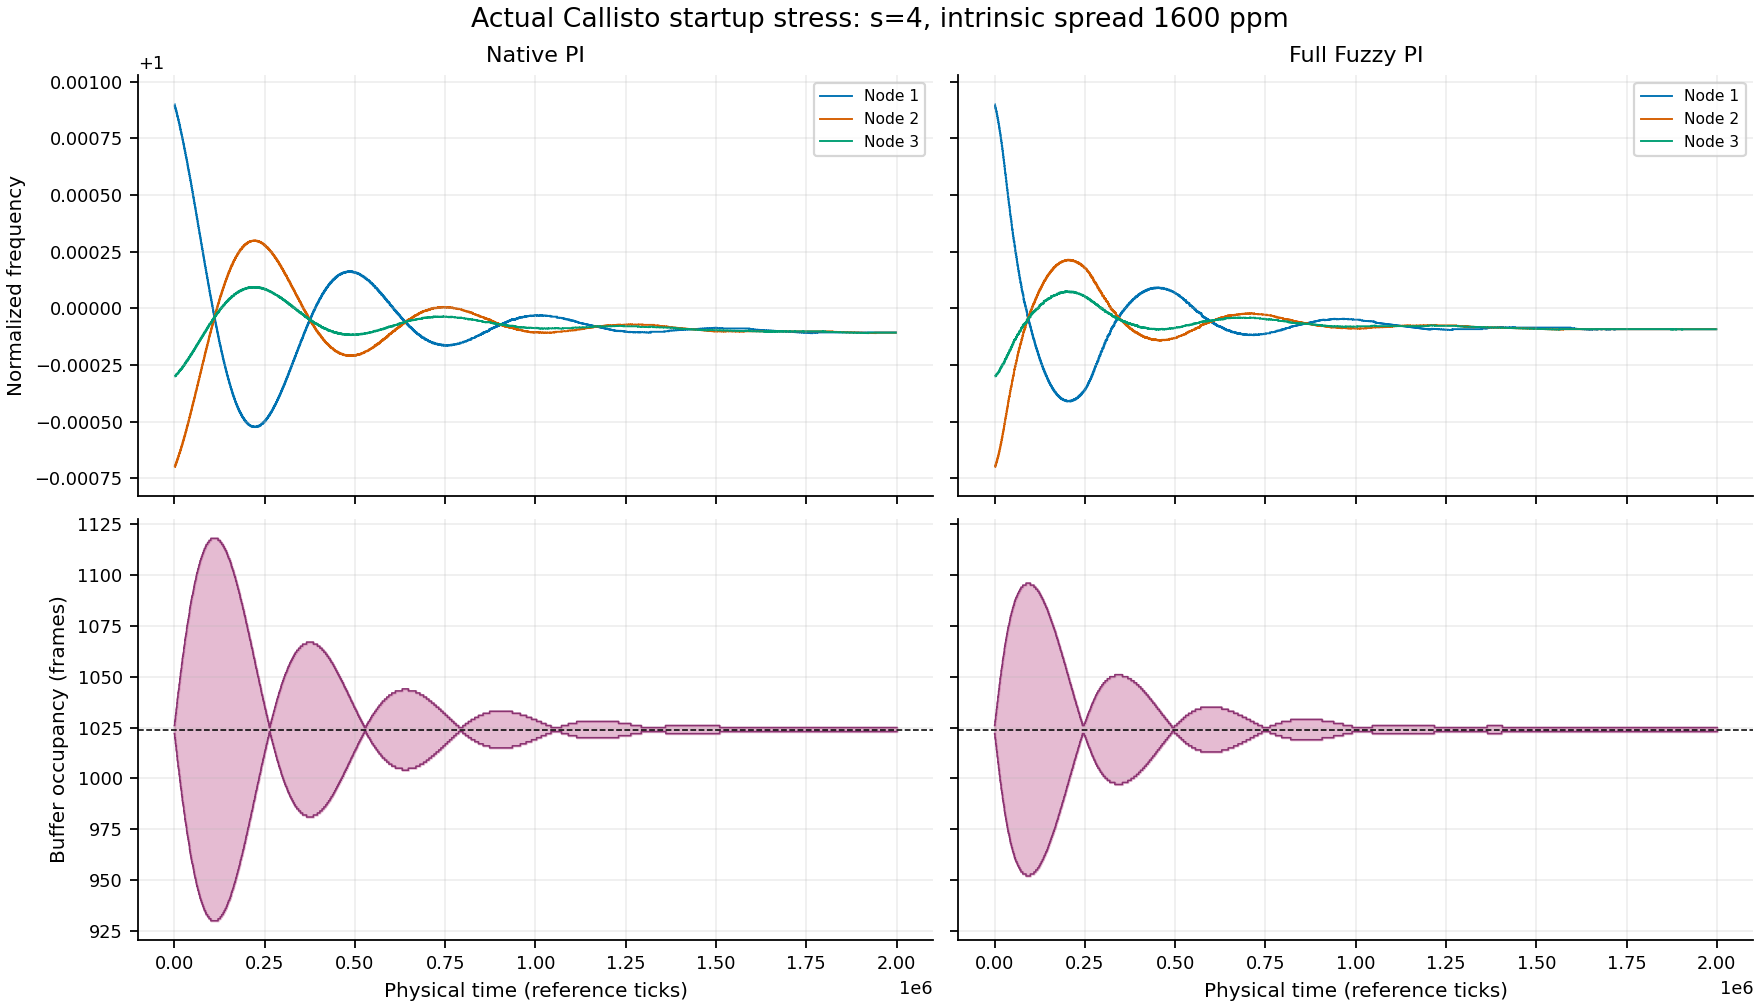
\includegraphics[width=0.97\textwidth]{images/evaluation_latest_20261103/actual_s4.png}
\caption{Actual continuous-phase Callisto startup at $s=4$ (1600 ppm),
with matched moderate coordinates. Upper panels show positive absolute
normalized frequencies using a $+1$ axis offset. Lower panels show the
minimum--maximum occupancy envelope across all receiving buffers, from
the complete crossing stream. Fuzzy reduces the maximum target
deviation from 94 to 72 frames over the stated startup horizon.}
\Description{PI and Fuzzy startup trajectories at the same frequency mismatch,
with absolute node frequencies and complete-event buffer-occupancy envelopes.}
\label{detail:fig:eval_startup_actual}
\end{figure*}

These observations show a smaller transient buffer demand at matched
gains, but do not transfer the reference theorem
to delayed, asynchronous, quantized execution. The recorded pairwise
spread remains a separate quantity. No hardware-based numerical
$\Delta_{\rm safe}$ is assumed; applying the reference spread corollary
would require an independently justified threshold exceeding $D(R)$.

\subsection{Equal-budget selection and independent random-latency tests}
\label{detail:subsec:eval_random}

\paragraph{Fixed search budget and selection.}
Each family uses the same 24-point grid,
\begin{align}
 k_p&\in\{1.5,2,2.5,3,4,6\}\times10^{-6},\nonumber\\
 k_i&\in\{1,2,5,10\}\times10^{-11}.
 \label{detail:eq:eval_gain_grid}
\end{align}
Fuzzy fixes $K_e=0.1$ and obtains $K_{\Delta e},K_u$ from the
calibration in Section~\ref{detail:sec:fpi_controller}; it receives no extra
shape-search dimension. Four training cases per candidate comprise
clean operation, a single-edge 20-tick delay increment lasting
$10^5$ ticks, and two random regimes using training seed 31001.
Both families therefore receive 96 evaluation slots. Four hash-verified
cached evaluations remain charged within the 192-slot total.
Nineteen PI and 22 Fuzzy candidates satisfy the same finite-run
admissibility requirements; all seven infeasible candidates are
retained without replacement.

Five training objectives are minimized separately: worst random-case
RMS, burst IAE, worst disturbance-window buffer excursion, peak absolute
common-frequency excursion from own clean, and worst mean command TV.
Each family's feasible Pareto set supplies a random-priority
representative, labeled $R$, and a burst-priority representative,
labeled $B$. The frozen lexicographic rule prioritizes random RMS for
$R$ and burst IAE for $B$, with the remaining objectives and candidate
identifier as declared tie breakers. One PI serves both priorities;
Fuzzy selects distinct representatives (Table~\ref{detail:tab:eval_selected_gains}).
Deduplication gives three candidates, without backfilling.

\begin{table*}[t]
\caption{Frozen representatives. The $k_p,k_i$ columns are native PI gains
for PI and calibrated PI coordinates for Fuzzy. $R$ and $B$ denote
random- and burst-priority selection; the candidates are not retuned on tests.}
\label{detail:tab:eval_selected_gains}
\centering
\begin{tabular}{@{}llrrrrr@{}}\toprule
Representative & Candidate & $k_p$ & $k_i$ & $K_e$ & $K_{\Delta e}$ & $K_u$\\\midrule
PI$_R$ = PI$_B$ & PI\_g05 & $2\times10^{-6}$ & $10^{-11}$ & --- & --- & ---\\
Fuzzy$_R$ & Fuzzy\_g02 & $1.5\times10^{-6}$ & $2\times10^{-11}$ & 0.1 & 7.499750 & $-1.638455\times10^{-5}$\\
Fuzzy$_B$ & Fuzzy\_g17 & $4\times10^{-6}$ & $10^{-11}$ & 0.1 & 39.998667 & $-8.192273\times10^{-6}$\\\bottomrule
\end{tabular}
\end{table*}

\paragraph{Untouched paired tests.}
Only after freezing selection are test profiles generated from seeds
41001--41030. All three candidates execute both original random
regimes and both held-out burst combinations, giving
$30\times2\times3+2\times3=186$ new actual runs. All 186 complete
and satisfy the declared normal-admissibility checks, with no
engineering QA errors or complete-event replay mismatches. No seed
pair is excluded. Archived M3 seeds are not reused as untouched tests.

The primary random comparison is Fuzzy$_R$ versus PI$_R$. Let $\ell$
index independent seeds. Report the paired mean difference and mean
of per-seed ratios,
\begin{align}
 \widehat d&=\frac1{30}\sum_{\ell=1}^{30}
       (R_{W,\ell}^{\rm Fuzzy_R}-R_{W,\ell}^{\rm PI_R}),\nonumber\\
 \widehat r&=\frac1{30}\sum_{\ell=1}^{30}
       R_{W,\ell}^{\rm Fuzzy_R}/R_{W,\ell}^{\rm PI_R}.
 \label{detail:eq:eval_paired_ratio}
\end{align}
The ratio is not the ratio of group means. Confidence intervals (CIs)
use 20000 paired-seed percentile-bootstrap resamples, with fixed
resampling seeds 58001/58002. Pointwise 95\% intervals accompany
each endpoint; a joint statement about the two original regimes also
uses nominal Bonferroni-adjusted 97.5\% intervals per regime.
Time points, edges and bootstrap draws are not independent replications.

\begin{table*}[t]
\caption{Untouched original-regime tests: 30/30 admissible pairs per row.
Controller RMS entries are seed means in ppm. Difference is Fuzzy$_R$
minus PI$_R$; ratios are means of paired ratios. Brackets give pointwise
95\% paired bootstrap intervals.}
\label{detail:tab:eval_random}
\centering
\begin{tabular}{@{}lrrll@{}}\toprule
Profile grid & PI$_R$ RMS & Fuzzy$_R$ RMS & Difference / ppm [CI] & Paired ratio [CI]\\\midrule
$T_c=1000$ & 4.61355 & 3.83949 & $-0.77406$ [$-0.80767$,$-0.73992$] & 0.83217 [0.82484,0.83964]\\
$T_c=10000$ & 4.65204 & 4.28718 & $-0.36486$ [$-0.43523$,$-0.29464$] & 0.92150 [0.90630,0.93672]\\\bottomrule
\end{tabular}
\end{table*}

Table~\ref{detail:tab:eval_random} and Figure~\ref{detail:fig:eval_random_primary}
show reductions in disagreement RMS at both tested profile grids.
The mean paired relative improvements are 16.78\% and 7.85\%.
The nominal family-adjusted difference intervals are
$[-0.81274,-0.73483]$ and $[-0.44451,-0.28407]$ ppm, also below zero.
This supports an advantage of the selected Fuzzy scheme under the
declared finite-grid budget, plant and two input regimes. Because
the selected coordinates differ between families, it does not
isolate a same-gain inference-only effect or establish globally
optimal PI/Fuzzy performance.

\begin{figure*}[t]
\centering
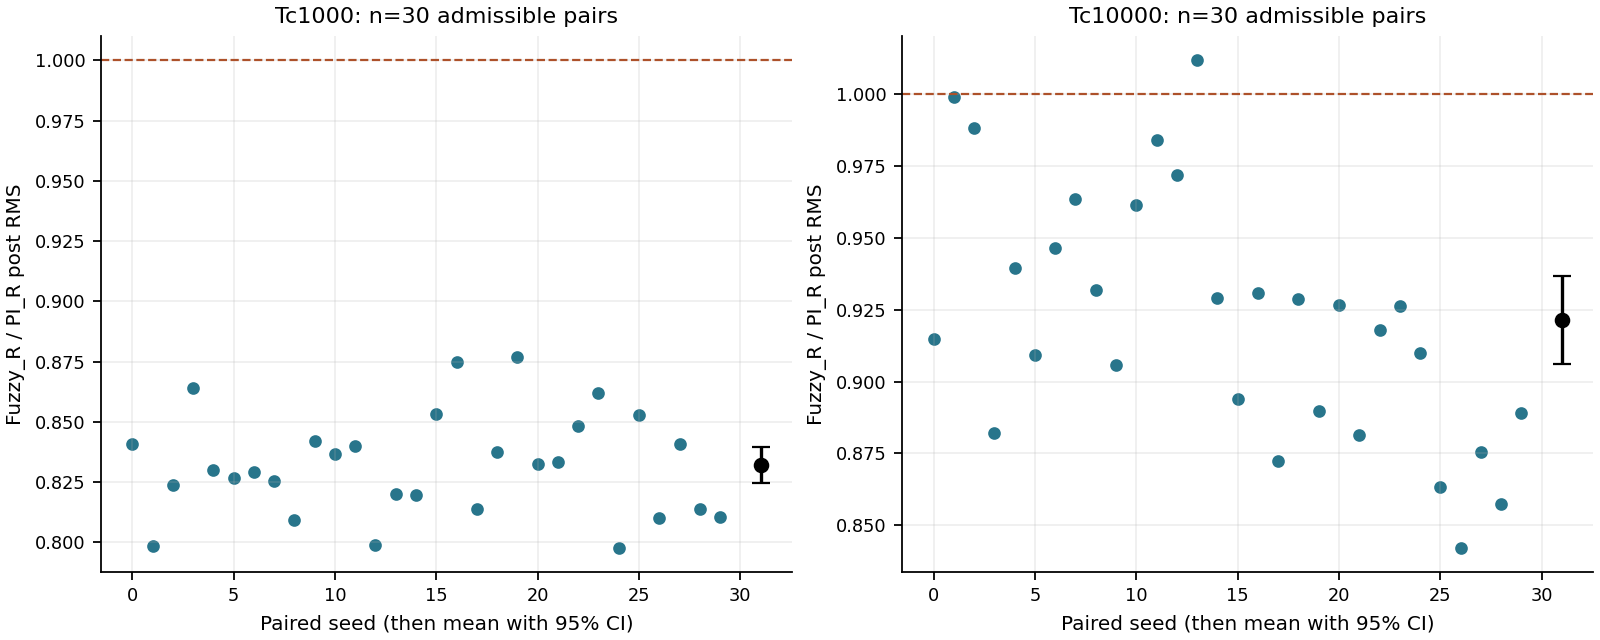
\includegraphics[width=0.97\textwidth]{images/evaluation_latest_20261103/paired_random_effects.png}
\caption{Independent paired Fuzzy$_R$/PI$_R$ RMS effects after equal-budget
selection. Each dot is one of 30 untouched seed pairs. The final black
marker is the mean paired ratio with a pointwise 95\% CI; the dashed
line denotes equal RMS. Individual seed outcomes and their aggregate
are both retained.}
\Description{Paired test-seed RMS ratios for profile intervals 1000 and
10000 ticks, with mean effects and bootstrap confidence intervals.}
\label{detail:fig:eval_random_primary}
\end{figure*}

\begin{figure*}[t]
\centering
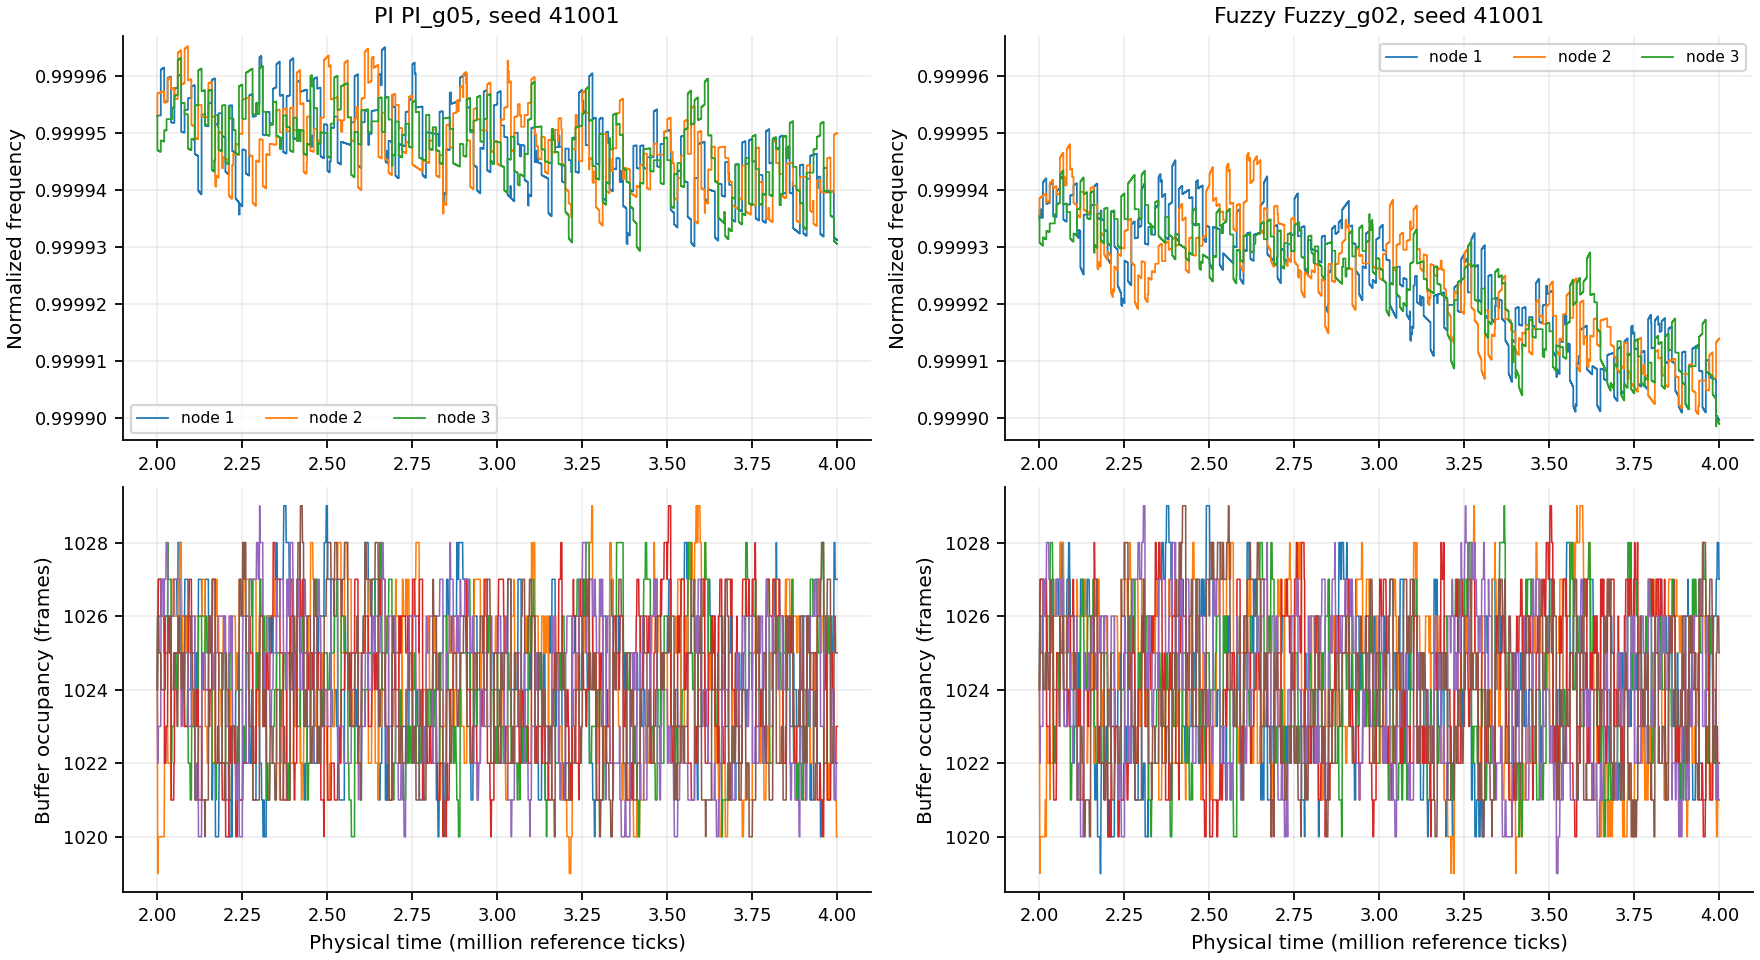
\includegraphics[width=0.97\textwidth]{images/evaluation_latest_20261103/raw_Tc10000.png}
\caption{Saved raw traces for the first held-out seed (41001) in the
$T_c=10000$ random experiment. Frequency uses held corrections and shared physical
time; buffer occupancy overview samples are for display. Reported
moments and buffer extrema instead use complete intervals and events.
The paired-seed statistics, rather than this one trace, support the
mean performance comparison.}
\Description{Shared-time node-frequency and buffer-occupancy
histories for the first held-out bounded-random delivery input.}
\label{detail:fig:eval_random_raw}
\end{figure*}

\paragraph{Activity and common-frequency cost.}
Mean per-node command TV decreases from 0.0102361 to 0.00782282 at
$T_c=1000$, and from 0.00112361 to 0.000906694 at $T_c=10000$
(PI$_R$ to Fuzzy$_R$). All selected candidates have at most six frames
of disturbance-window target deviation. However, Fuzzy$_R$ has larger
magnitude mean tail common-frequency shifts from own clean:
$-61.420$ versus $-15.692$ ppm, and $-31.933$ versus $-15.384$ ppm.
Thus reduced relative disagreement and command activity do not
imply improved absolute-frequency regulation. No absolute-frequency
reference loop is present.

\subsection{Held-out bursts and slower delivery changes}
\label{detail:subsec:eval_burst}

\paragraph{Burst-priority validation.}
The two predetermined held-out combinations are a 10-tick desired
delay increment lasting $10^4$ ticks on channel $2\to3$, and a
40-tick increment lasting $10^5$ ticks on $3\to1$, both beginning
at $2\times10^6$. They are distinct from the training combination.
For the larger burst, Fuzzy$_B$ lowers post-onset IAE from
$8.19241\times10^6$ to $3.62317\times10^6$ ppm$\cdot$ticks,
approximately 55.8\%, while matching the 40-frame buffer excursion.
Table~\ref{detail:tab:eval_heldout_bursts} retains both deterministic cases:
the improvement depends on the burst combination rather than holding
for every tested burst. These two cases do not supply seed-level CIs.

\begin{table}[t]
\caption{Both held-out burst-priority cases over
$[2\times10^6,4\times10^6)$. IAE is in $10^6$ ppm$\cdot$ticks;
buffer excursion is in frames. $A$ and $D$ denote desired delay
increment and its duration, respectively.}
\label{detail:tab:eval_heldout_bursts}
\centering
\begin{tabular}{@{}lrrrr@{}}\toprule
 & \multicolumn{2}{c}{IAE} & \multicolumn{2}{c}{Buffer excursion}\\
Case & PI$_B$ & Fuzzy$_B$ & PI$_B$ & Fuzzy$_B$\\\midrule
$A=10,D=10^4$ & 0.265814 & 0.352614 & 11 & 11\\
$A=40,D=10^5$ & 8.192410 & 3.623166 & 40 & 40\\\bottomrule
\end{tabular}
\end{table}

\paragraph{Ramp--hold--ramp inputs.}
A separate registered study freezes the selected gains and applies
a 20-tick delay increment on channel $1\to2$ using rise/fall times
$T_r\in\{10^4,10^5\}$ and hold times
$T_h\in\{10^5,10^6\}$. The four combinations all run to
$5.2\times10^6$ ticks. The end of the falling ramp is
$t_{\rm off}=2\times10^6+2T_r+T_h$; each case has its own
$[t_{\rm off},t_{\rm off}+2\times10^6)$ recovery window and
same-horizon clean counterfactual. A larger constant delay plateau
does not mean delivery stops throughout that plateau. The ramp
instead gives feedback time to act while the delivery imbalance forms.

For $T_r=10^5$, maximum buffer deviations are 19 frames for PI,
18 for Fuzzy$_R$ and 17 for Fuzzy$_B$. The slower formation of the
disturbance therefore provides another observed buffer-margin
benefit. Frequency RMS favors PI across the four ramp combinations,
and strict own-clean recovery is censored in all 12 ramp records.
Different disturbance durations are not pooled into a raw-IAE ranking;
these data support a resource/frequency tradeoff, not a faster-settling claim.

\paragraph{Separately registered slow-random confirmation.}
The slower grid $T_c=100000$ uses new seeds 51001--51030, unchanged
selected gains, the same bounded recursion, and
$W=[2\times10^6,5\times10^6)$ with tail
$[4.6\times10^6,5\times10^6)$. Each trace has 30 complete
profile blocks, which are not independent statistical replicates.
The study includes 105 matrix slots: three long-clean cases,
12 ramps and 90 random cases. Four matrix slots reuse qualified
pilot runs; 101 new main runs plus six pilots give 107 unique actual
runs. All matrix slots pass profile, nominal-prefix and event-replay
checks, with no excluded confirmation seed pairs.

This confirmation bounds the applicability of the original-regime
advantage: the mean paired Fuzzy$_R$/PI$_R$ RMS ratio is 1.33312
with pointwise 95\% CI [1.30337,1.36219], using 20000 paired
bootstrap resamples and fixed seed 59001. The mean paired difference
is $+1.53215$ ppm [1.39578,1.66175]. Slower variation alone therefore
does not extend the selected controller's RMS advantage. This confirmation
delimits the two original-regime benefits without changing their
registered primary endpoints or the frozen controller selection.

\subsection{Connection between analysis and measured benefits}
\label{detail:subsec:eval_support}

The evidence supports two benefits. First, nonlinear analysis at
matched gain coordinates proves a strict headroom improvement for the
prescribed fluid reference; actual matched-gain startup tests also show
smaller measured excursions at three fixed initial mismatches. Second,
equal-budget, independent selection yields lower disagreement RMS and
mean command activity in two held-out random regimes, while the
burst-priority representative reduces IAE in the larger held-out burst.
These are distinct statements with different gains, assumptions and
observation windows.

Their scope is explicit: common-frequency shift remains a cost, the
small burst and slower delivery tests delimit performance, and finite
actual records do not certify all-time safety or convergence. The
experiments do not establish a general safe-set inclusion, a globally
optimal comparator, payload-level functional logical synchrony, or
hardware energy savings. Positive phase progress and buffer compliance
show normal model execution; they are not a functional refinement proof.
Within these limits, the combined analysis and tests provide both a
mechanistic reason and independent empirical evidence for considering
the proposed Fuzzy PI law when transient buffer use and
disturbance-dependent synchronization performance matter.


% =====================================================================
% HISTORICAL EVALUATION BEFORE LATEST RESULTS -- ALL LINES COMMENTED
% Preserved for review; old fixed-preset tables/plots are not compiled.
% This archive does not replace the current confirmation-scope summary.
% =====================================================================
% % Evaluation assembled from completed evidence only, 2026-11-03.
% % No new Callisto runs, tuning/selection or PDF compilation is required.
% \section{Evaluation}
% \label{detail:sec:evaluation}
% 
% The evaluation addresses three questions. First, does the implementation
% respect the PI calibration and initialization derived in
% Section~\ref{detail:sec:fpi_controller}? Second, are the reference-model
% calculations consistent with the implemented nonlinear rule law? Third,
% how does the full Fuzzy controller compare with fixed PI baselines under
% post-centering delivery disturbances in continuous-phase Callisto?
% These questions require separate evidence: implementation equivalence,
% reference-model consistency, and finite-horizon performance do not
% establish the same claim.
% 
% \subsection{Evidence groups and comparison design}
% \label{detail:subsec:eval_design}
% 
% We use three completed actual-Callisto campaigns, denoted M0, M2 and M3,
% and separate fluid-reference calculations. M0 comprises six PI/linear-
% counterpart pairs, or 12 actual runs. M2 comprises four actual runs:
% PI and full Fuzzy, each with a clean trace and a single-edge latency
% burst. M3 comprises 180 actual validation runs: 30 independent paired
% seeds, two random-latency regimes and three fixed controllers. Six M3
% pilot runs are separate from the 180-run validation and are not treated
% as independent test replications. Reference calculations are not added
% to the actual-Callisto run count.
% 
% The primary performance comparison is moderate PI against the full
% Fuzzy law calibrated to its PI gain coordinates. M3 additionally includes
% a prespecified stronger PI candidate. All candidates are frozen within
% these campaigns. The linear surface $F_0$ is used only for the M0
% implementation check and explicitly labeled same-input diagnostics;
% M2 and M3 execute the full 25-rule nonlinear law. Axis matching controls
% scales and update conventions, but is not an assertion that either
% candidate is the best independently tuned controller.
% 
% \subsection{Continuous Callisto setup and delivery disturbances}
% 
% M2 and M3 use the continuous oscillator phases, local-clock scheduling
% and integer receiving-buffer counts described in
% Section~\ref{detail:sec:fpi_controller}. Table~\ref{detail:tab:eval_setup} gives their
% common configuration. Reported token counts represent counted frames
% in this model. There is no shared physical controller grid in
% these actual runs. The fixed native integration scale is
% $h=p/\omega_{\rm base}$, with the same convention in the calibrated
% Fuzzy controller. The initial intrinsic-frequency spread is 400 ppm of
% the normalized frequency unit.
% 
% \begin{table*}[t]
% \caption{Common configuration of the aligned burst and random-latency experiments.
% Time is measured in physical reference ticks unless specified as local ticks.}
% \label{detail:tab:eval_setup}
% \centering
% \begin{tabular}{@{}ll@{}}\toprule
% Parameter & Value\\\midrule
% Network & Three-node bidirectional triangle; six receiving buffers\\
% Intrinsic frequencies $\omega^u$ & $(1.0002,0.9998,0.9999)^\top$\\
% Initial phases; implementation base frequency & $0.1$ at every node; $\omega_{\rm base}=29999/30000$\\
% Capacity; initial occupancy; target & $C=2048$; $\beta_e(0)=\beta_e^*=1024$ frames\\
% Initial in-flight frames; delayed-run marking & 20 per channel; 1044 in the recorded convention\\
% Nominal physical path delay & 20\\
% Polling; control-execution delay & $p=1000$; $d_{\rm ctrl}=10$ local ticks\\
% Moderate PI $(k_p,k_i)$ & $(2\times10^{-6},5\times10^{-11})$\\
% Stronger fixed PI, M3 only & $(4\times10^{-6},5\times10^{-11})$\\
% Full Fuzzy $(K_e,K_{\Delta e},K_u)$ & $(0.1,3.9998666667,-4.0961365379\times10^{-5})$\\
% Execution policy & $u_{\max}=0.01$; shared guards enabled; reserve zero; no anti-windup\\
% Optional mechanisms & Observer and supervisory mode switching disabled\\
% Horizon; disturbance onset & $4\times10^6$; $t_{\rm on}=2\times10^6$\\\bottomrule
% \end{tabular}
% \end{table*}
% 
% \paragraph{Burst after nominal centering.}
% In M2, desired send-time latency on one directed channel, identified as
% $1\to2$ in the runtime configuration, changes from 20 to 40 during
% $[2\times10^6,2.1\times10^6)$ and returns to 20 afterwards. All other
% channels remain at 20. Each controller has its own clean counterfactual
% with latency 20 throughout. A controller's burst and clean histories
% match before onset, so their subsequent difference isolates the effect
% of the delivery disturbance for that controller. The nominal states
% of PI and Fuzzy are not required to be identical to each other.
% 
% \paragraph{Bounded random latency.}
% M3 uses fixed physical profile-update grids $T_c=1000$ and $10000$,
% independently of the unchanged controller polling period. For each
% generated link profile the bounded recursion is
% \begin{align}
%  z_0&=5\varepsilon_0,\nonumber\\
%  z_m&=r_z z_{m-1}+(1-r_z)5\varepsilon_m,
%  \qquad r_z=e^{-1},\quad\varepsilon_m\sim\mathcal U[-1,1],
%  \label{detail:eq:eval_random_profile}
% \end{align}
% with desired delay $20+z_m\in[15,25]$ after onset. Here $m$ indexes
% profile updates, not controller measurements. The designation $T_c$
% refers to the profile grid, not an exactly measured correlation time.
% Before onset, including negative-time prehistory, delay is 20. Seeds
% 20001--20030 are independent validation replications; pilot seed 1001
% is excluded. For each seed and regime, all three controllers receive
% identical externally generated profile content.
% 
% Both disturbance families use the declared causal running-maximum
% arrival envelope. Frame order is retained and a delay decrease can
% release an ordered batch. No finite serialization-rate model, frame
% dropout or application-payload experiment is included. These are
% specified transport stress models rather than claims about arbitrary
% network traffic.
% 
% \subsection{Metrics, windows and finite-run admissibility}
% \label{detail:subsec:eval_metrics}
% 
% \paragraph{Disagreement and absolute frequency.}
% For the instantaneous common frequency $\bar\omega(t)=n^{-1}\sum_i\omega_i(t)$,
% define
% \begin{align}
%  \sigma_\omega(t)&=\sqrt{\frac1n\sum_i[\omega_i(t)-\bar\omega(t)]^2},\nonumber\\
%  s(t)&=10^6\sigma_\omega(t)/\omega_{\rm unit},\qquad\omega_{\rm unit}=1.
%  \label{detail:eq:eval_disagreement_amplitude}
% \end{align}
% Thus $s$ is an instantaneous across-node root-mean-square (RMS)
% amplitude in parts per million (ppm). Its normalization is the fixed
% unit frequency, not $\omega_{\rm base}$ or the reference ramp frequency
% used in Section~\ref{detail:sec:btd_reference}. For $W=[t_s,t_e)$ with duration
% $T_W=t_e-t_s$, report
% \begin{align}
%  R_W&=\sqrt{T_W^{-1}\int_W s(t)^2\,dt},\nonumber\\
%  I_W&=\int_W s(t)\,dt,\qquad P_W=\sup_{t\in W}s(t).
%  \label{detail:eq:eval_frequency_metrics}
% \end{align}
% The recorded integral absolute error (IAE) is $I_W$, the integral of
% this nonnegative RMS amplitude. It is not the integral of the mean
% absolute node deviation. Moments are integrated over complete held-
% frequency intervals using physical-duration weights, not uniform
% averages of controller updates.
% 
% These quantities must also be distinguished from the pairwise spread
% $\Delta_\omega(t)=\max_i\omega_i(t)-\min_i\omega_i(t)$ of
% Section~\ref{detail:sec:btd_reference}. Cauchy--Schwarz gives
% $\Delta_\omega(t)\le\sqrt{2n}\,\sigma_\omega(t)$, but a window RMS
% does not bound a pointwise transient by itself. We retain positive-
% frequency checks and common-frequency diagnostics separately. For M2,
% a supplementary descriptive spread calculation uses the already saved
% shared-time frequency intervals; it is not a new simulation or a
% preregistered primary endpoint.
% 
% \paragraph{Buffer excursion and control activity.}
% Measured buffer excursion and remaining headroom are
% \begin{align}
%  B_W^{\rm obs}&=\max_e\sup_{t\in[t_s,t_e]}|\beta_e(t)-\beta_e^*|,\nonumber\\
%  H_W^{\rm obs}&=\min_e\inf_{t\in[t_s,t_e]}
%                      \min\{\beta_e(t),C-\beta_e(t)\}.
%  \label{detail:eq:eval_buffer_metrics}
% \end{align}
% Every integer phase crossing and ordered arrival is reconstructed.
% Simultaneous events are grouped under the frozen convention, and
% buffer extrema include the right-endpoint state. Display samples are
% not the source of peak or moment statistics. Conservative reference
% certificates are not substituted for measured extrema.
% Mean per-node command total variation (TV) is
% \begin{equation}
%  \mathrm{TV}_W=\frac1n\sum_i
%        \sum_{k:\,t_s\le t^a_{i,k}\le t_e}|u_{i,k}-u_{i,k-1}|.
%  \label{detail:eq:eval_tv}
% \end{equation}
% Activity uses inclusive endpoints in the frozen protocol; adjacent
% subwindow activities must not be added without handling their shared
% boundary. All evaluated M2/M3 runs have zero recorded saturation, so
% requested and applied command increments coincide. TV is a command-
% activity measure, not measured hardware energy or computational cost.
% 
% \paragraph{Windows and recovery.}
% The primary disturbance window is $[2\times10^6,4\times10^6)$.
% M2 additionally separates burst ON and post-OFF intervals at
% $t_{\rm off}=2.1\times10^6$. Before onset, both M2 controllers and all
% M3 cases pass three consecutive $10^5$-tick nominal windows: disagreement
% RMS at most 2 ppm, each buffer's absolute mean bias at most two frames
% and standard deviation at most one frame, common-frequency temporal
% standard deviation at most 1 ppm and three-window mean range at most
% 1 ppm, with positive frequencies/progress and no intervention. These
% are finite engineering centering criteria, not exact equilibrium.
% 
% M2 component recovery requires these criteria in three consecutive
% post-OFF windows. Strict recovery additionally requires the window-mean common
% frequency to return within 2 ppm of that controller's own clean
% trajectory over the same physical-time window. A missing qualifying return by
% $4\times10^6$ is right-censored; it is neither zero recovery time nor
% proof of permanent nonrecovery. M3 uses $[3.6\times10^6,4\times10^6)$
% for tail diagnostics. The separate M2 memory decomposition below uses
% $[3.7\times10^6,4\times10^6)$.
% 
% \subsection{Implementation equivalence and reference consistency}
% \label{detail:subsec:eval_implementation_reference}
% 
% M0 varies polling over 100 and 1000 local ticks, initial frequency
% spread over 35 and 400 ppm, and includes capacity/target settings
% $(2048,1024)$, $(512,128)$ and $(512,384)$ across its six matched pairs.
% All pairs use constant path delay 20, execution delay 10 and a
% $2\times10^5$-tick horizon. Target-centered percentages are used for
% non-midpoint targets. Across 19,800 paired updates, the maximum
% requested/applied correction difference is $5.29\times10^{-18}$.
% Physical and data phases coincide at all evaluated union knots, with
% identical measurement vectors and saved-time buffer counts. No guard
% intervention or saturation is recorded. This supports the implemented
% calibration, integration order and constructor treatment of
% Proposition~\ref{detail:prop:fpi_equivalence}; it is not a nonlinear-Fuzzy
% performance result or a general runtime-equivalence proof.
% 
% Separate previously completed reference calculations call the original
% 25-rule Fuzzy update directly, rather than advance the plant with a
% sector surrogate. Two trajectories use moderate and stronger gain
% coordinates, each with 2000 post-bootstrap updates. For the moderate
% configuration corresponding to Section~\ref{detail:sec:btd_reference}, the
% observed maximum fluid buffer deviation is approximately 17.314056818
% frames, maximum $|X|+|Y|$ is 0.090130790, and maximum absolute correction
% is $3.21398377\times10^{-4}$. There are no observed stepwise
% contraction-envelope violations; frequencies remain in
% $[0.9998,1.0002]$ including startup. These numerical checks are
% consistent with the reference certificate, but the all-time guarantee
% and strict PI comparison come from the interval-prefix and certified-
% tail argument of Theorem~\ref{detail:thm:btd_headroom}, not from a finite
% floating-point trajectory. The reference marking is 1024; the delayed
% actual runs' marking is 1044.
% 
% \subsection{Response to a post-centering latency burst}
% \label{detail:subsec:eval_burst}
% 
% Table~\ref{tab:eval_burst} reports the aligned moderate-gain comparison.
% Figure~\ref{fig:eval_burst_overview} shows the shared-time frequency,
% buffer and latency traces, including the clean counterfactuals.
% Fuzzy reduces RMS-amplitude IAE by 1.864\% and mean command TV by
% 15.938\%. Its disagreement RMS is 0.096\% higher, instantaneous RMS
% peak is 2.396\% higher, and target-referenced buffer excursion is one
% frame larger. These endpoints establish a tradeoff at this deterministic
% operating point, not a uniform disturbance-rejection advantage.
% 
% \begin{table*}[t]
% \caption{M2 metrics over $[2\times10^6,4\times10^6)$ unless stated otherwise.
% Lower is preferable except for buffer headroom. The spread row is a
% supplementary descriptive calculation; no engineering spread threshold
% was predeclared for these runs.}
% \label{tab:eval_burst}
% \centering
% \begin{tabular}{@{}lrr@{}}\toprule
% Metric & Moderate PI & Full Fuzzy\\\midrule
% Disagreement RMS $R_W$ / ppm & 9.67059 & 9.67988\\
% Instantaneous RMS peak $P_W$ / ppm & 32.59447 & 33.37534\\
% RMS-amplitude IAE $I_W/(10^6\ \mathrm{ppm\cdot ticks})$ & 9.94254 & 9.75722\\
% Supplementary peak pairwise spread / ppm & 69.14830 & 70.89161\\
% Buffer excursion $B_W^{\rm obs}$ / frames & 20 & 21\\
% Minimum lower / upper buffer headroom / frames & 1004 / 1017 & 1003 / 1017\\
% Mean command TV / $10^{-4}$ & 2.62204 & 2.20415\\
% Largest command increment / $10^{-5}$ & 4.10000 & 4.21763\\
% Peak common-frequency difference from own clean / ppm & 60.61864 & 61.26423\\
% Component entry / confirmation after OFF / $10^6$ ticks & 0.8 / 1.1 & 0.8 / 1.1\\
% Strict own-clean recovery by the horizon & Censored & Censored\\
% Full-run buffer excursion, including startup / frames & 24 & 21\\\bottomrule
% \end{tabular}
% \end{table*}
% 
% \begin{figure*}[t]
% \centering
% 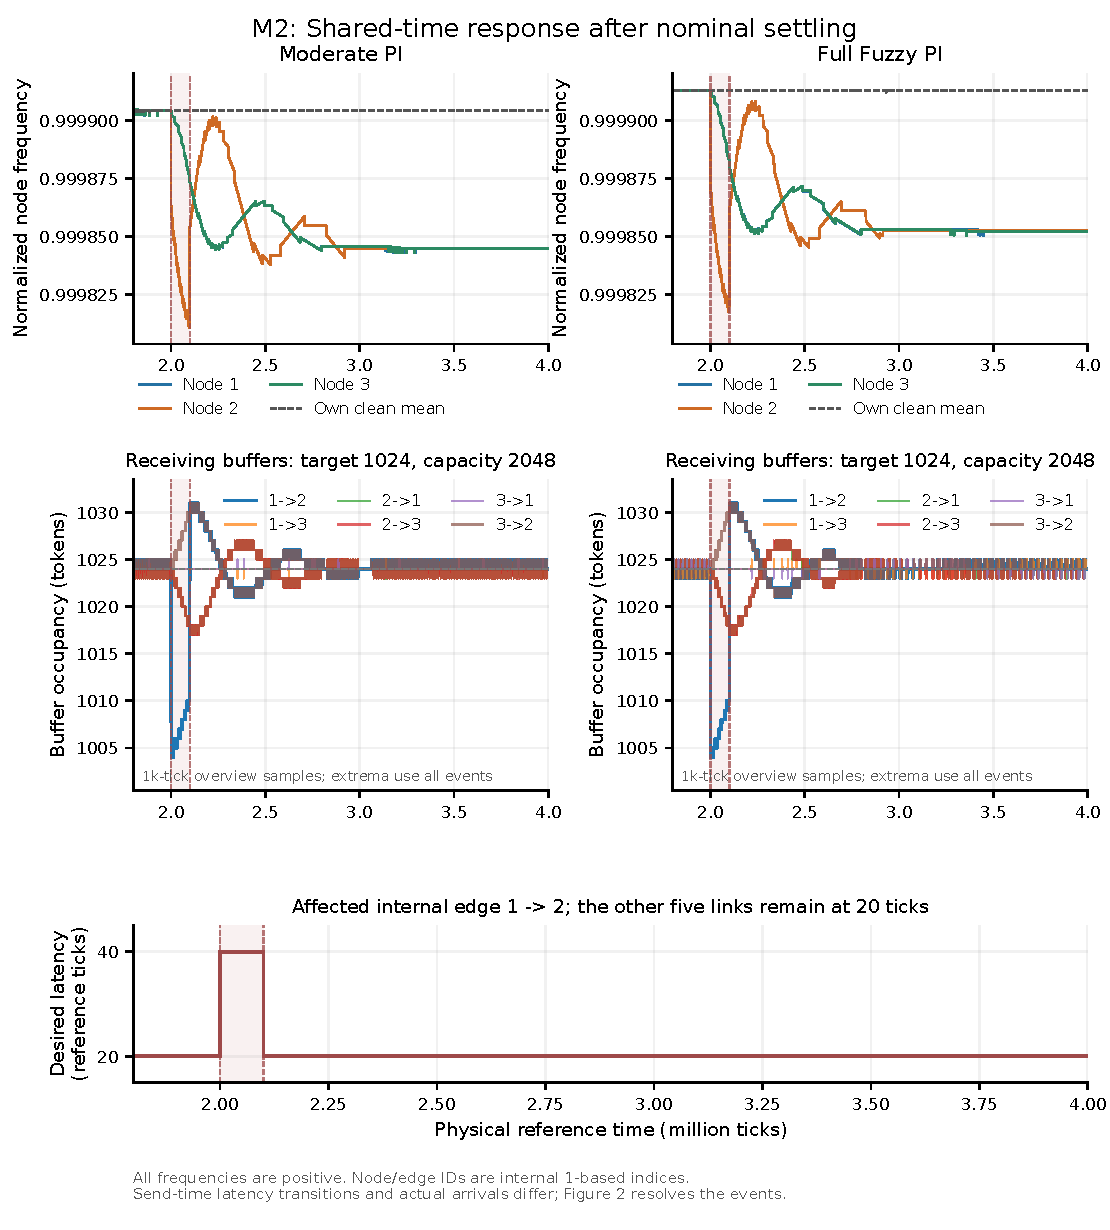
\includegraphics[width=0.97\textwidth]{images/evaluation_20261103/m2_shared_time_response.pdf}
% \caption{Aligned post-centering burst experiment. Continuous-phase Callisto
% uses the fixed moderate PI coordinates and their full-Fuzzy calibration.
% Both controllers have their own clean counterfactual. Desired latency on
% one directed channel changes from 20 to 40 during
% $[2\times10^6,2.1\times10^6)$. Frequency histories use held corrections;
% buffer overview samples are for display, while reported buffer statistics
% come from the complete reconstructed event stream.}
% \Description{Shared-time overview of node frequencies, six receiving-buffer
% occupancies, and the imposed path-latency burst for PI and Fuzzy PI.}
% \label{fig:eval_burst_overview}
% \end{figure*}
% 
% Both controllers remain within capacity with positive frequency and
% continuing logical phase progress, without recorded guard or saturation
% intervention. Including startup, the full-run maximum deviation is
% 24 frames for PI and 21 for Fuzzy. This is a favorable Fuzzy endpoint
% for that full window, whereas the post-onset peaks are 20 and 21.
% Changing the window changes the ranking, so neither figure is used as
% a replacement for the other. Capacities are far from exhaustion.
% 
% Both first enter the window-qualified component recovery band at
% $2.9\times10^6$ and confirm it at $3.2\times10^6$. Thus the experiment
% does not show faster Fuzzy settling under this criterion. Strict
% own-clean recovery is censored for both. In the memory-diagnostic
% tail, the common-frequency changes relative to own clean are
% $-59.40198$ ppm for PI and $-60.51069$ ppm for Fuzzy. A stationary
% common frequency, frequency agreement between nodes, return to own
% clean, and return to frequency one are different properties.
% 
% \subsection{Observed nonlinear mechanism and the first buffer peak}
% \label{subsec:eval_mechanism}
% 
% The M2 rule replay agrees with the full nonlinear implementation.
% All sampled Fuzzy input pairs remain in $\Omega_5$, with disturbance-window
% maximum $|X|+|Y|=2.001888$. The central identity of
% Proposition~\ref{detail:prop:fpi_central} therefore applies to those observed
% updates. However, this trajectory does not stay in the smaller
% $\Omega_1$ input diamond used by the reference example. This is not
% evidence of a sector violation or instability; it is another reason,
% besides asynchrony, delay and quantization, that the example's
% invariant-region certificate is not a certificate for this actual burst.
% 
% The Section~\ref{detail:sec:fpi_controller} decomposition into proportional,
% integral-like and accumulated nonlinear-residual terms reproduces the
% requested correction with maximum residual is approximately
% $6.46\times10^{-18}$. In the diagnostic tail, the Fuzzy own-clean
% common-frequency shift decomposes into
% \begin{equation}
%  -60.51069=-57.61859-2.89210\quad\mathrm{ppm},
%  \label{eq:eval_memory_accounting}
% \end{equation}
% where the two terms are the linear integral-like contribution and
% nonlinear memory; the proportional contribution is zero. PI's
% $-59.40198$ ppm shift is its integral contribution. This is exact
% same-trajectory accounting up to numerical arithmetic, not an
% independently evolving $F_0$ closed-loop ablation or a unique causal
% explanation of the physical common frequency.
% 
% Figure~\ref{fig:eval_mechanism} also resolves the first buffer peak.
% PI and Fuzzy first attain their disturbance-window maximum target deficits at
% ON$+39.105$ and ON$+40.731$ ticks, whereas their first changed commands
% relative to own clean occur at ON$+155.216$ and ON$+155.841$.
% At the respective first extrema, clean/burst occupancies are
% 1024/1004 for PI and 1023/1003 for Fuzzy. Both same-time
% clean-minus-burst deficits are therefore 20 frames: target deficits of
% 20 and 21 combine that delivery deficit with clean-state offsets of
% zero and one. Consequently the first attainment is not a measurement
% of post-burst feedback effectiveness. The minimum is revisited later;
% we do not claim that every peak instance precedes feedback.
% 
% \begin{figure*}[t]
% \centering
% 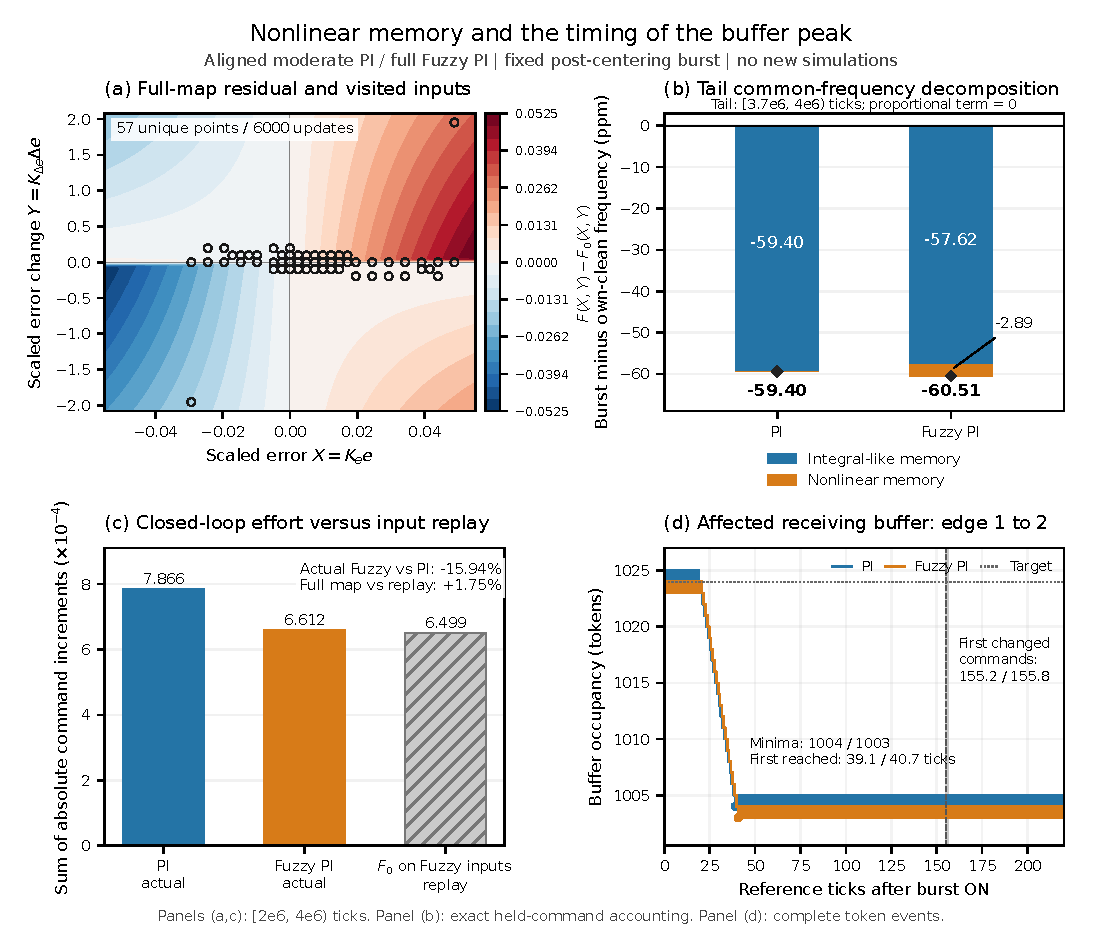
\includegraphics[width=0.97\textwidth]{images/evaluation_20261103/m2_nonlinear_memory.pdf}
% \caption{Nonlinear mechanism diagnostics reusing the four M2 runs.
% The panels show the exact central residual $F-F_0$, common-frequency
% memory accounting, command activity and complete early buffer events.
% The hatched $F_0$ activity bar is a replay on Fuzzy's measured inputs,
% not a third closed-loop experiment. The residual surface is multiplied
% by negative $K_u$ in the controller. The memory panel uses
% $[3.7\times10^6,4\times10^6)$; activity uses the main disturbance
% window. First peak attainment precedes the first changed command, but
% the peak can be revisited after feedback begins.}
% \Description{Four panels connecting Fuzzy rule residuals, stored correction
% memory, command total variation, and early buffer depletion timing.}
% \label{fig:eval_mechanism}
% \end{figure*}
% 
% \subsection{Independent paired random-latency validation}
% \label{detail:subsec:eval_random}
% 
% All 180 M3 validation runs are normal-admissible, with zero saved-state
% mismatches in complete-event replay. Table~\ref{detail:tab:eval_random}
% summarizes the primary endpoint. The ratio estimand is
% \begin{equation}
%  \widehat r=\frac1{30}\sum_{s=1}^{30}
%        \frac{R_{W,s}^{\rm Fuzzy}}{R_{W,s}^{\rm PI}},
%  \label{detail:eq:eval_paired_ratio}
% \end{equation}
% where $s$ indexes independent seeds. It is not the ratio of the two
% group means. Pointwise 95\% confidence intervals (CIs) use 20,000
% paired-seed percentile-bootstrap resamples with fixed resampling seeds.
% Time points, edges and bootstrap draws are not independent experimental
% replications. Regimes are analyzed separately; the intervals do not
% provide simultaneous multiple-endpoint coverage. There are no excluded
% pairs in the reported comparisons.
% 
% \begin{table*}[t]
% \caption{M3 primary disturbance-window disagreement RMS. Controller entries
% are means over 30 seeds in ppm. Ratios are means of paired seed ratios
% with pointwise 95\% CIs. A ratio below one favors Fuzzy.}
% \label{detail:tab:eval_random}
% \centering
% \begin{tabular}{@{}lrrrll@{}}\toprule
% Profile grid & PI moderate & PI stronger & Fuzzy & Fuzzy/moderate [CI] & Fuzzy/stronger [CI]\\\midrule
% $T_c=1000$ & 4.911 & 9.347 & 5.856 & 1.1925 [1.1722,1.2150] & 0.6266 [0.6155,0.6389]\\
% $T_c=10000$ & 6.696 & 9.699 & 7.152 & 1.0679 [1.0624,1.0736] & 0.7365 [0.7184,0.7554]\\\bottomrule
% \end{tabular}
% \end{table*}
% 
% \begin{figure*}[t]
% \centering
% 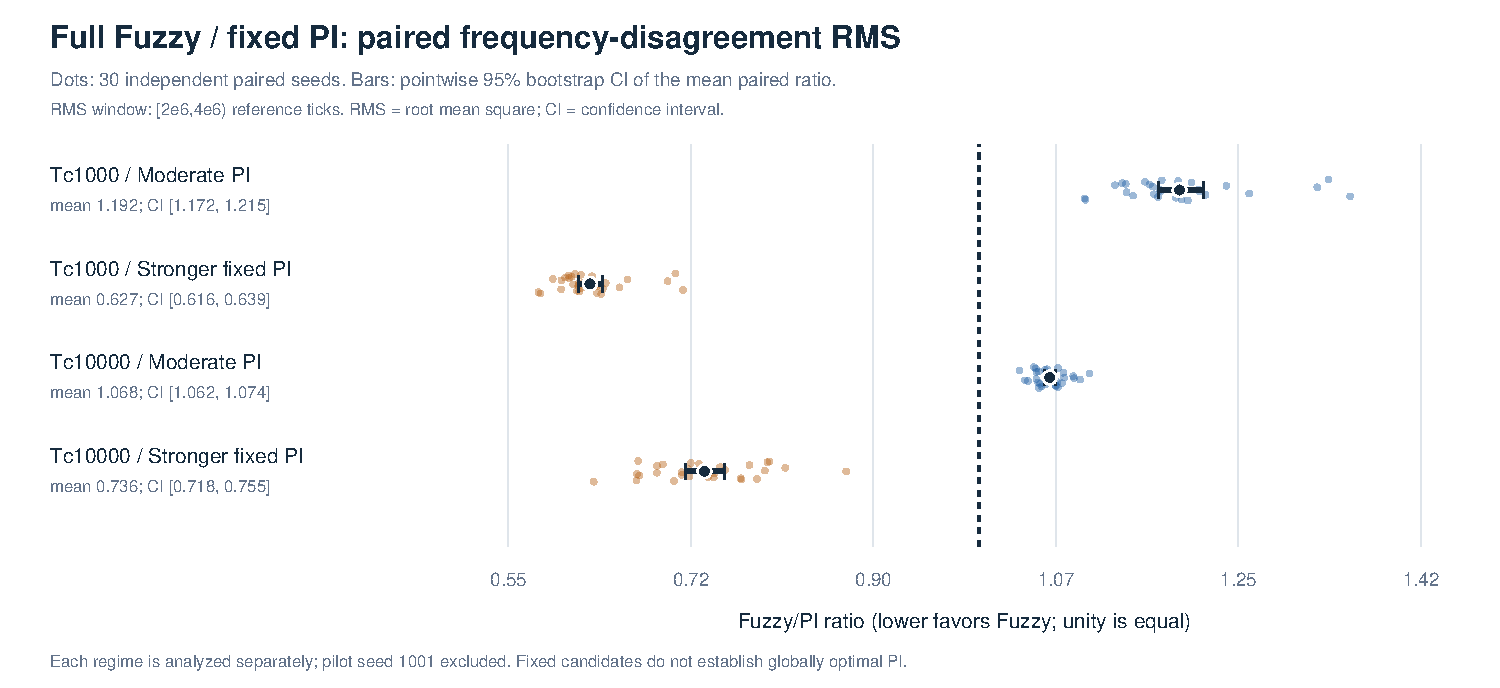
\includegraphics[width=0.97\textwidth]{images/evaluation_20261103/m3_primary_paired_effects.pdf}
% \caption{Independent paired random-latency validation: primary disagreement
% RMS and paired Fuzzy/PI effects for two physical profile grids. Thirty
% seeds per regime are shared across the three fixed controllers. The
% moderate comparator is the primary axis-matched PI baseline; stronger
% PI is a separate fixed candidate. Ratios and pointwise confidence
% intervals follow the paired-seed protocol, rather than resampling
% correlated controller updates.}
% \Description{Primary random-latency disagreement results and paired effects
% against moderate and stronger fixed PI for thirty seeds per regime.}
% \label{detail:fig:eval_random_primary}
% \end{figure*}
% 
% Relative to moderate PI, Fuzzy has higher RMS in all 30 seeds of each
% regime: mean paired increases are 19.245\% and 6.791\%. The lower
% RMS relative to stronger fixed PI is comparator-specific; moderate PI
% already has lower RMS than Fuzzy, so that comparison does not establish
% an inherent advantage of fuzzy inference over suitable PI tuning.
% The frozen random-latency hypothesis of lower disagreement RMS is
% therefore not supported against the primary baseline in these regimes.
% 
% Within the disturbance windows, all runs have at most seven frames of
% actual target deviation and at least 1017 frames of lower/upper
% headroom. These extrema exclude startup. They establish finite-run
% admissibility in this interior operating region, not a larger Fuzzy
% safe set. The random result also does not extend the M2 TV reduction:
% mean paired Fuzzy/moderate TV ratios are 1.03045 and 1.03153.
% Figure~\ref{fig:eval_random_secondary} retains buffer, effort and
% common-frequency diagnostics. Mean tail common-frequency shifts from
% each controller's pre-disturbance level are approximately
% $-156.682$ versus $-72.576$ ppm at $T_c=1000$, and $-76.540$
% versus $-67.816$ ppm at $T_c=10000$ (Fuzzy versus moderate PI).
% These finite-horizon shifts and trends are reported separately from
% relative synchronization; no absolute-frequency loop is present.
% 
% \begin{figure*}[t]
% \centering
% 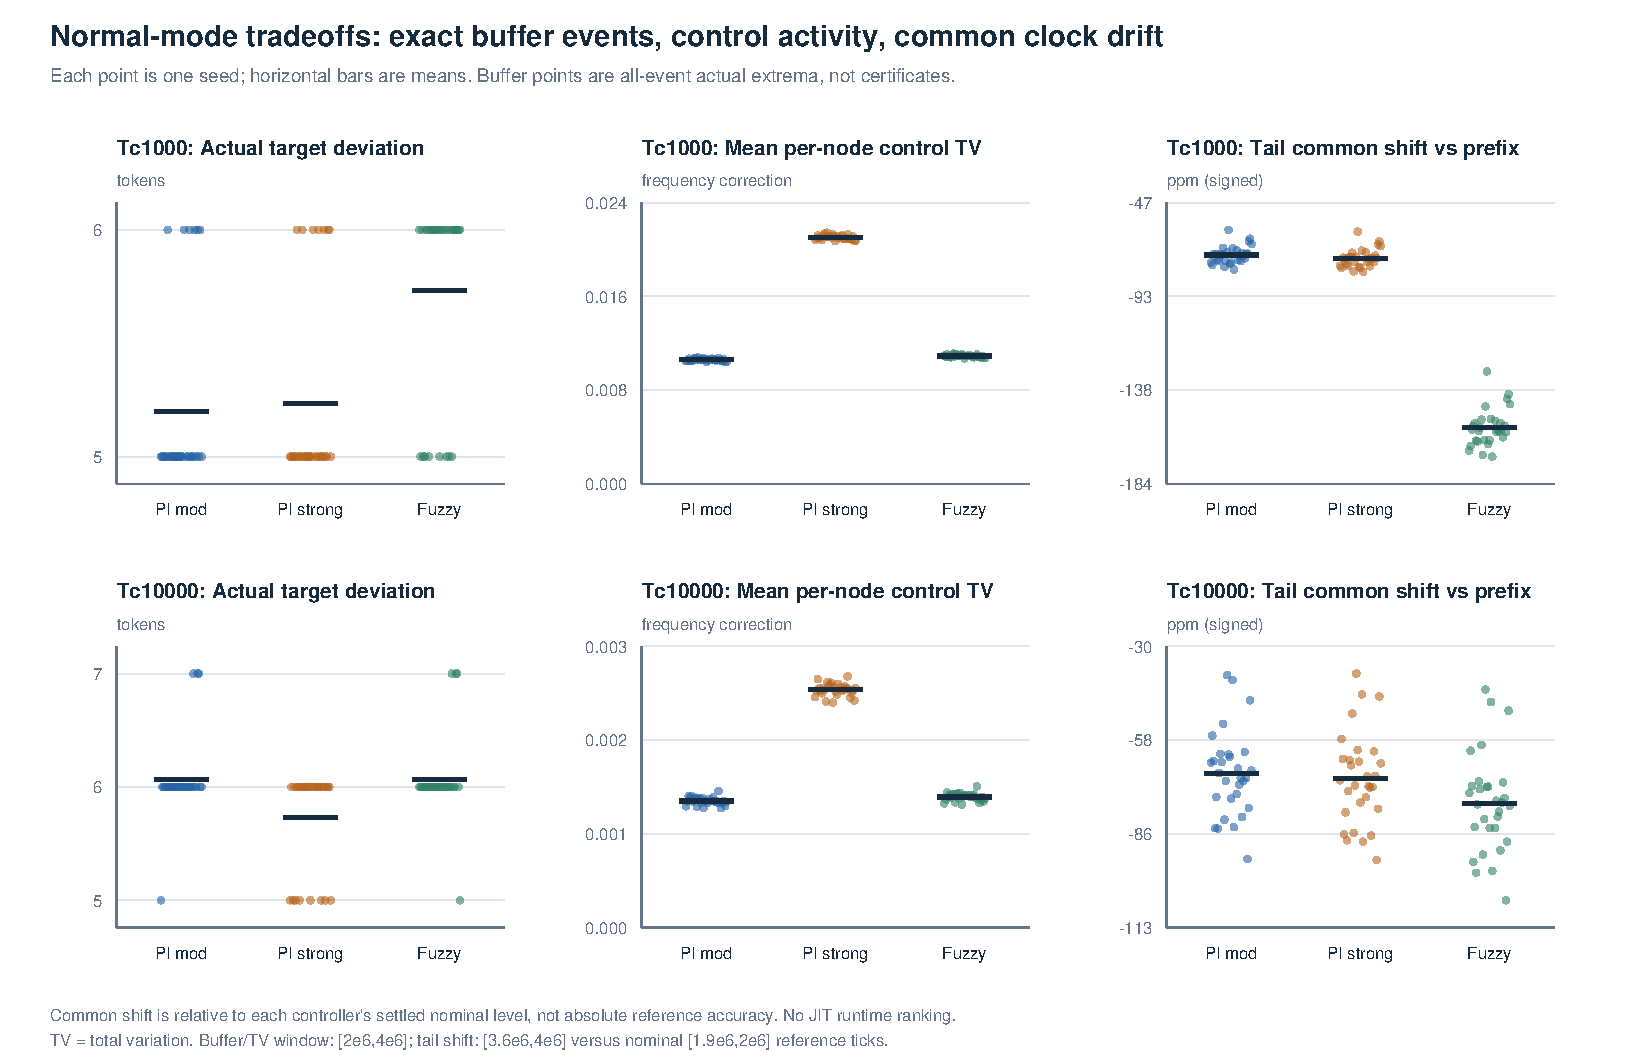
\includegraphics[width=0.97\textwidth]{images/evaluation_20261103/m3_buffer_effort_drift.pdf}
% \caption{Secondary M3 diagnostics over the declared windows: complete-event
% buffer excursions, command activity and common-frequency shift.
% The same 30 paired seeds underlie each regime; additional endpoints
% do not create additional independent replications. Buffer extrema
% refer to the disturbance window, not the startup trajectory.}
% \Description{Buffer, control activity and common-frequency diagnostics
% complementing the primary random-latency synchronization metric.}
% \label{fig:eval_random_secondary}
% \end{figure*}
% 
% \subsection{What the completed evaluation establishes}
% \label{detail:subsec:eval_support}
% 
% The evidence supports the implementation-consistent PI calibration,
% the exact nonlinear mechanism on observed M2 inputs, and the
% conditional reference-model buffer-headroom theorem. Actual Callisto
% demonstrates endpoint-dependent response shaping: a smaller full-run
% buffer excursion and lower post-burst IAE/TV at the stated M2 point,
% alongside higher post-onset peaks and no faster component recovery.
% The independent M3 study limits any general random-jitter advantage
% claim for the frozen controller. These outcomes are consistent with
% the paper's conditional mechanism-and-tradeoff formulation; they do
% not support uniform Fuzzy superiority.
% 
% The completed actual campaigns do not test the boundary of the
% reference invariant set. Their large buffer reserves cannot substitute
% for certified-safe, uncertified-but-observed-safe and failed cases
% around a common boundary. Nor do finite observations prove
% infinite-horizon safety or the reference theorem's optional
% frequency-spread tolerance in asynchronous delayed execution.
% Observed phase progress and capacity compliance support normal model
% execution; application-payload correctness and a formal refinement
% proof of logical synchrony are outside this evaluation.
% 
% Finally, these are fixed-controller comparisons, not a completed
% equal-budget tuning/held-out-test study. A separate preregistered
% tuning campaign has not completed its audit, selection and untouched
% tests; its partial results are excluded from the present performance
% tables. The evaluation also provides no P/GABA comparison, switched
% FFP or observer result, dropout recovery, serialized-link hardware
% test, or meaningful controller runtime/energy ranking. Consequently,
% practical adoption beyond the reported operating points remains an
% empirical question even though the reference-model headroom benefit
% is mathematically established.
